\documentclass[conference]{IEEEtran}
\IEEEoverridecommandlockouts
% The preceding line is only needed to identify funding in the first footnote. If that is unneeded, please comment it out.
\usepackage{cite}
\usepackage{amsmath,amssymb,amsfonts}
\usepackage{algorithmic}
\usepackage{graphicx}
\usepackage{textcomp}
\usepackage{xcolor}
\usepackage{tikz}

\usetikzlibrary{zx-calculus}


\def\BibTeX{{\rm B\kern-.05em{\sc i\kern-.025em b}\kern-.08em
    T\kern-.1667em\lower.7ex\hbox{E}\kern-.125emX}}
\begin{document}

\title{ZX-Calculus}

\author{
    \IEEEauthorblockN{ Manuel Lerchner}
    \IEEEauthorblockA{
        \textit{Technical University of Munich}\\
        Munich, Germany}
}

\maketitle

\begin{abstract}
    ZX-Calculus is a graphical language which extends classical quantum circuits by splitting up logic gates into even smaller building blocks. Those building blocks are called spiders and are represented by colored nodes in a graph. Together with edges connecting those nodes, they form a ZX-diagram. Using a set of rewrite rules, ZX-diagrams can be transformed into each other. This allows for a more intuitive way of reasoning about the optimization of quantum circuits, as there are fewer rewrite rules to remember than in the classical logic gate model. In this paper, I will introduce the ZX-Calculus and its rewrite rules, as well as some of its applications. I will give a special
\end{abstract}

\begin{IEEEkeywords}
    quantum computing, ZX-Calculus, quantum circuits, circuit optimization
\end{IEEEkeywords}

\section{Introduction}

ZX-Calculus has been kickstarted by Coecke and Duncan in 2008 \cite{Coecke2007graphicalcalculus}. Since then, it has been used to prove a lot of interesting results in quantum computing. It used in the field of Measurement Based Quantum Computing (MBQC) \cite{duncan2012graphical}. Recently \cite{vandewetering2020zxcalculus} it has found wide application in quantum circuit optimization and verification.

\section{Introduction to ZX-Calculus}

A ZX-diagram is a graph consisting of nodes and edges. The nodes are called spiders and are colored either green or red. Additionally, they may carry a phase value $\alpha \in [0, 2\pi)$. Spiders are visuallized in the following way:


\vspace{5pt}
\begin{ZX}
    \leftManyDots{n}  \zxZ{\alpha} \rightManyDots{m}
\end{ZX}

\vspace{5pt}


\begin{ZX}
    \leftManyDots{n}  \zxX{\alpha} \rightManyDots{m}
\end{ZX}
\vspace{5pt}


Here $n$ and $m$ are the number of incoming and outgoing edges, respectively. The phase value $\alpha$ is optional and can be omitted if it is zero.

It is important to remember that each spider represents a linear map from $n$ to $m$ qubits. This linear maps can be directly calculated using the following formulas:

\vspace{5pt}
\zx{\leftManyDots{n}  \zxX{\alpha} \rightManyDots{m}} $\equiv |\underbrace{0\dots 0}_{m}\rangle \langle \underbrace{0\dots0}_{n}| + e^{i\alpha}|\underbrace{1\dots1}_{m}\rangle \langle \underbrace{1\dots1}_{n}|$

\vspace{5pt}
\begin{ZX}
    \leftManyDots{n}  \zxZ{\alpha} \rightManyDots{m}
\end{ZX} $\equiv |\underbrace{+\dots +}_{m}\rangle \langle \underbrace{+\dots+}_{n}| - e^{i\alpha}|\underbrace{-\dots-}_{m}\rangle \langle \underbrace{-\dots-}_{n}|$
\vspace{5pt}

By just using single spiders, we can already represent a lot of quantum gates. The most important ones are shown in figure \ref{fig:spiders}. Note that in ZX-Calculus we ignore the global scalar factor of a quantum gate

\subsection*{Verifying some Unitary Gates}

Let's verify that the Pauli-Z gate and the Pauli-X gate can indeed be represented by the spiders shown in figure \ref{fig:spiders}.


\begin{align}
    \begin{ZX}[ampersand replacement=\&]
        \zxN{} \rar \&[\zxwCol] \zxZ{\pi} \rar \&[\zxwCol] \zxN{}
    \end{ZX}
     & \equiv |\underbrace{0\dots 0}_{1}\rangle \langle \underbrace{0\dots0}_{1}| + e^{i\pi}|\underbrace{1\dots1}_{1}\rangle \langle \underbrace{1\dots1}_{1}| \\
     & \equiv
    |0\rangle \langle 0| - |1\rangle \langle 1|                                                                                                                \\
     & \equiv
    \begin{pmatrix}
        1 \\
        0 \\
    \end{pmatrix}
    \begin{pmatrix}
        1 & 0 \\
    \end{pmatrix}
    - \begin{pmatrix}
          0 \\
          1 \\
      \end{pmatrix}
    \begin{pmatrix}
        0 & 1 \\
    \end{pmatrix}                                                                                                                                             \\
     & \equiv
    \begin{pmatrix}
        1 & 0  \\
        0 & -1 \\
    \end{pmatrix}                                                                                                                                             \\
     & \equiv Z
\end{align}


\begin{figure}
    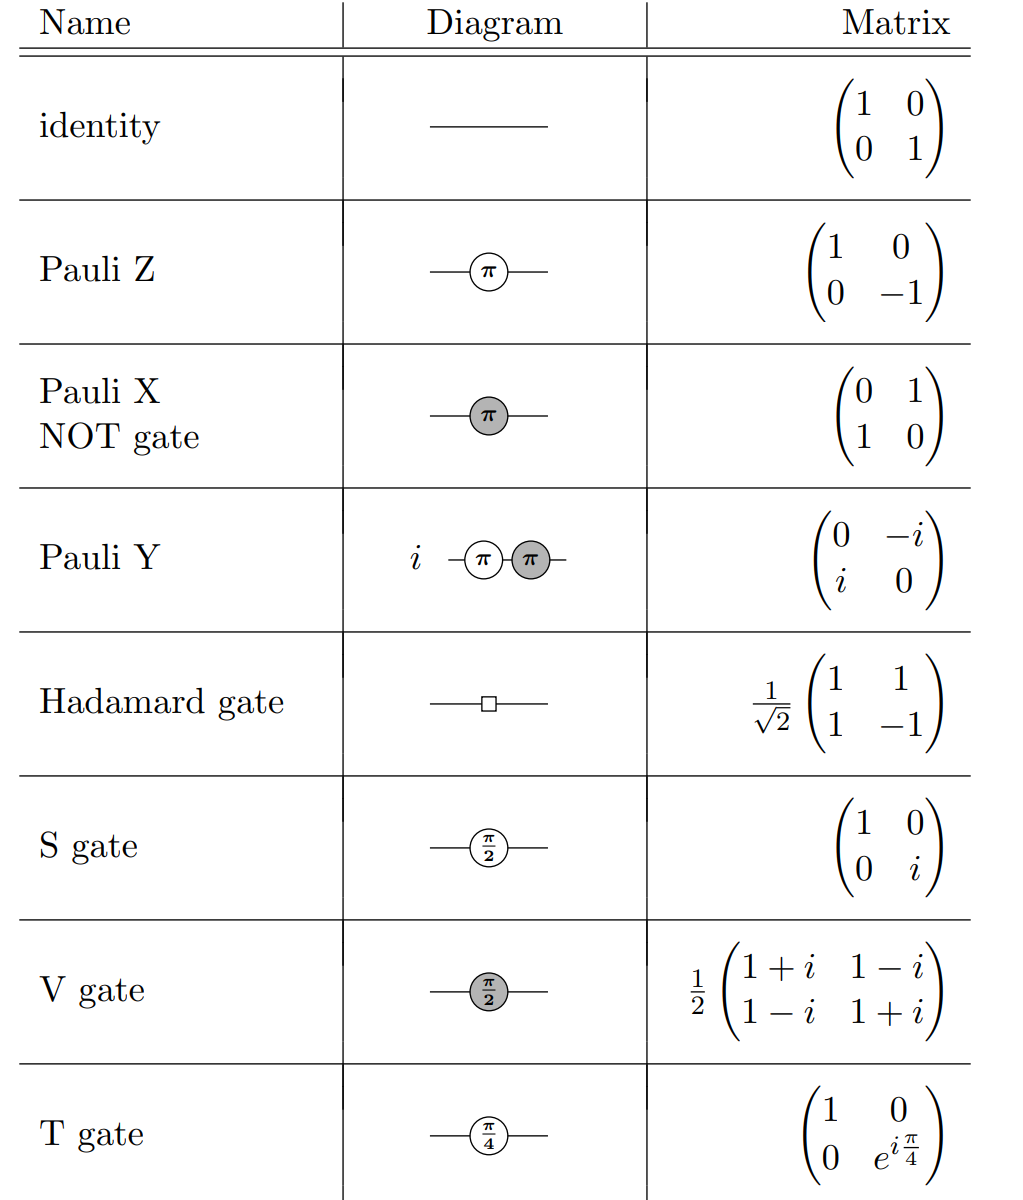
\includegraphics[width=\linewidth]{images/single_spider_unitaries.png}
    \caption{Spiders representing quantum gates
            {\cite{vandewetering2020zxcalculus}[P.87]}}
    \label{fig:spiders}
\end{figure}














\section{Motivation}


\section{Problem Statement}

\section{Solution}

\section{Evaluation}

\section{Results}

\section{Future Work}

\section{Conclusion}



\bibliographystyle{plain}
\bibliography{refs}



\end{document}
